\chapter{General Information}
\label{sec:general_information}
VentPro is a website for displaying information and controlling the essential parameter of an ABB ventilation system remotely via the web interface.
This user manual describes the VentPro website and guides the user through its functions. It does not provide detailed technical information about the web application - for this information the technical program documentation should be consulted. It is recommended to read all the information provided. For additional information, please contact the VentPro development team.\\



\chapter{Login}
\label{sec:login}

\begin{figure}[h]
\centering
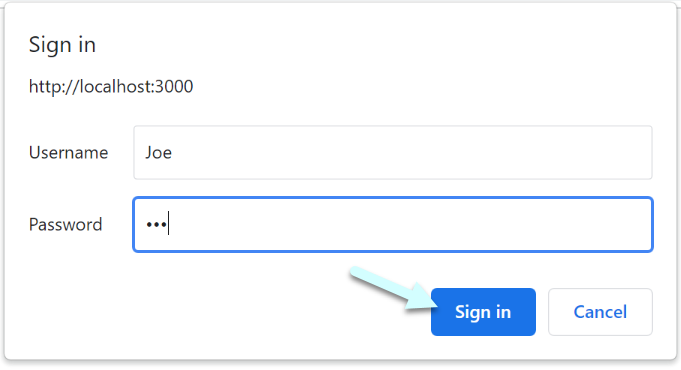
\includegraphics{img/Picture1}
\caption{Login form}
\label{fig:picture_1}
\end{figure}
\vspace{0.3cm}

\begin{enumerate}[wide,  labelwidth=0.3cm,  labelindent=0pt, leftmargin=0.5cm]
\item In order to access the website type “localhost:3000” in the address line of your internet browser and press enter.
\item A login window pops up in the upper part of the screen and asks for username and password. The admin, which created your account, should have provided you with this information.
\item Write the given username and password in the respective textbox and press enter or click the “Sign in” button (figure \ref{fig:picture_1}).
\item The login was successful if the “Control Panel” page is displayed as shown in figure \ref{fig:picture_2}.
\item If you type in wrong credentials, the pop-up window asks again for your username and password.
\item When clicking the “Cancel” button to terminate the login activity, the message “Error: You are not authenticated!” is displayed.
\end{enumerate}

\color{red}
Note! If it is your first time using this website it is recommended to change the password, which the admin provided.
\color{black}



\chapter{Navigation menu}
\label{sec:navigation_menu}

\begin{figure}[h]
\centering
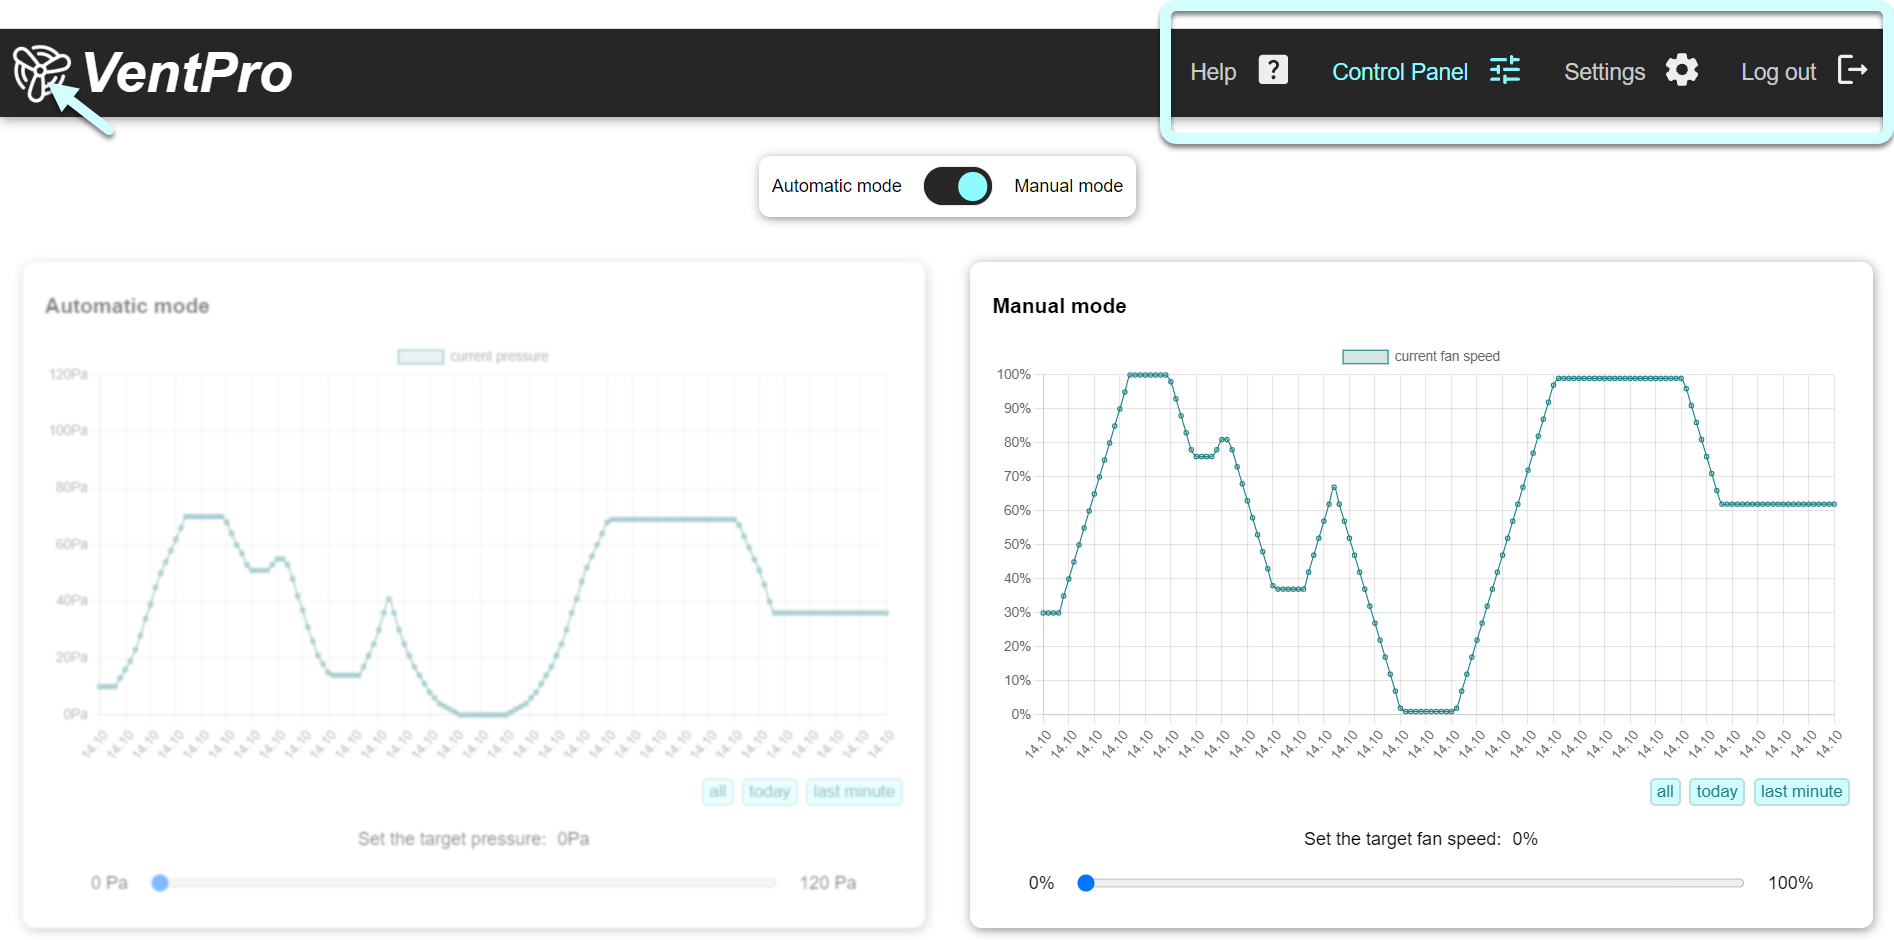
\includegraphics[width=1.0\textwidth]{img/Picture2}
\caption{Control panel}
\label{fig:picture_2}
\end{figure}
\vspace{0.3cm}

Every page has a navigation menu at the top of the screen. It contains the following elements: “Help” “Control Panel“, “Settings” and “Log out”. By clicking one of the buttons the user is directed to the respective page. On the left hand side of the navigation menu the logo of VentPro can be clicked to direct the user to the main page, which is the “Control Panel” page (figure \ref{fig:picture_2}).
 
 
 
\chapter{Help}
\label{sec:help}

The “Help page” displays important information for the website’s users in a frequently asked question style. The questions are divided into two sections, “Control Panel” and “Sections”. By clicking “control panel” and “settings” written above the questions and in lowercase, the user is directed to the respective section. Each question is displayed in a box with a plus sign in the right corner. By pressing the plus sign the box expands and the answer to the question appears (figure \ref{fig:picture_3}).

\vspace{0.5cm}
\begin{figure}[h]
\centering
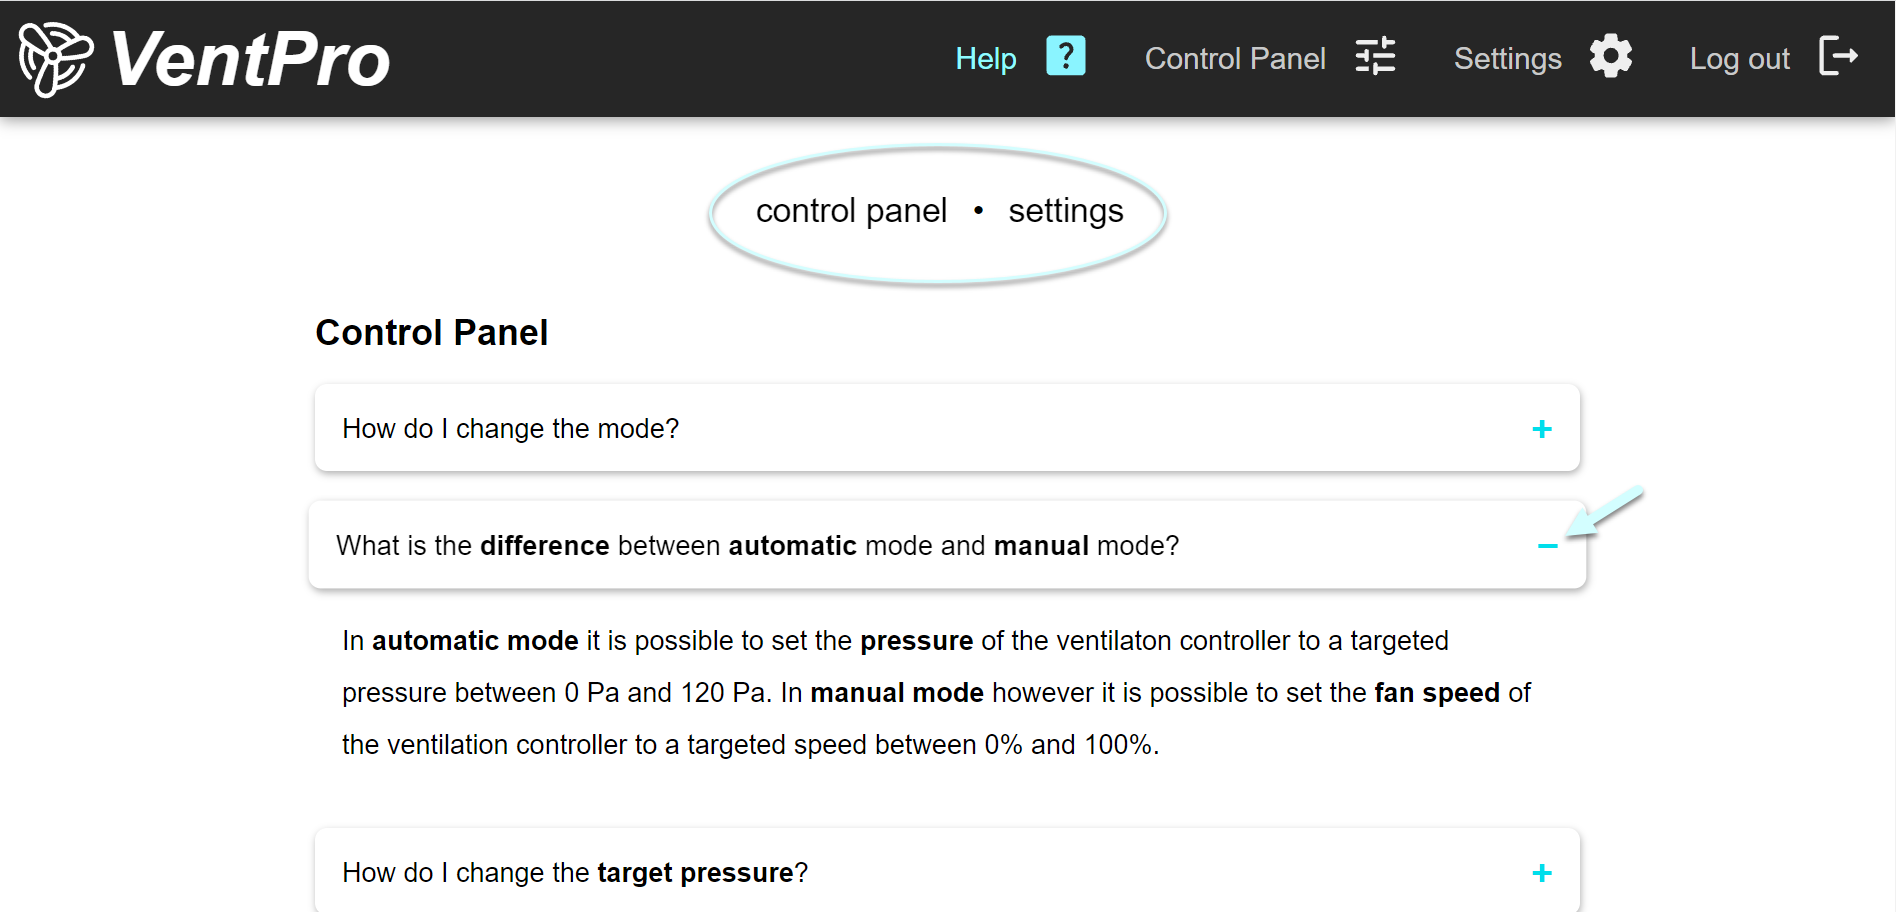
\includegraphics[width=1.0\textwidth]{img/Picture3}
\caption{Help page}
\label{fig:picture_3}
\end{figure}



\chapter{Control Panel}
\label{sec:control_panel}

This chapter describes the “Control Panel page”, which provides the main functionalities for controlling the ventilation. The page displays two graphs, one for the automatic and the other one for the manual mode of the ventilator. There is also a button to switch between these two modes. Each mode is blurred when not in use. The graphs visualize data recorded from the ventilation controller. Furthermore, you can interact with the ventilator by changing its fan speed or pressure.


\section{Automatic mode}
\label{sec:automatic_mode}

\begin{figure}[h]
\centering
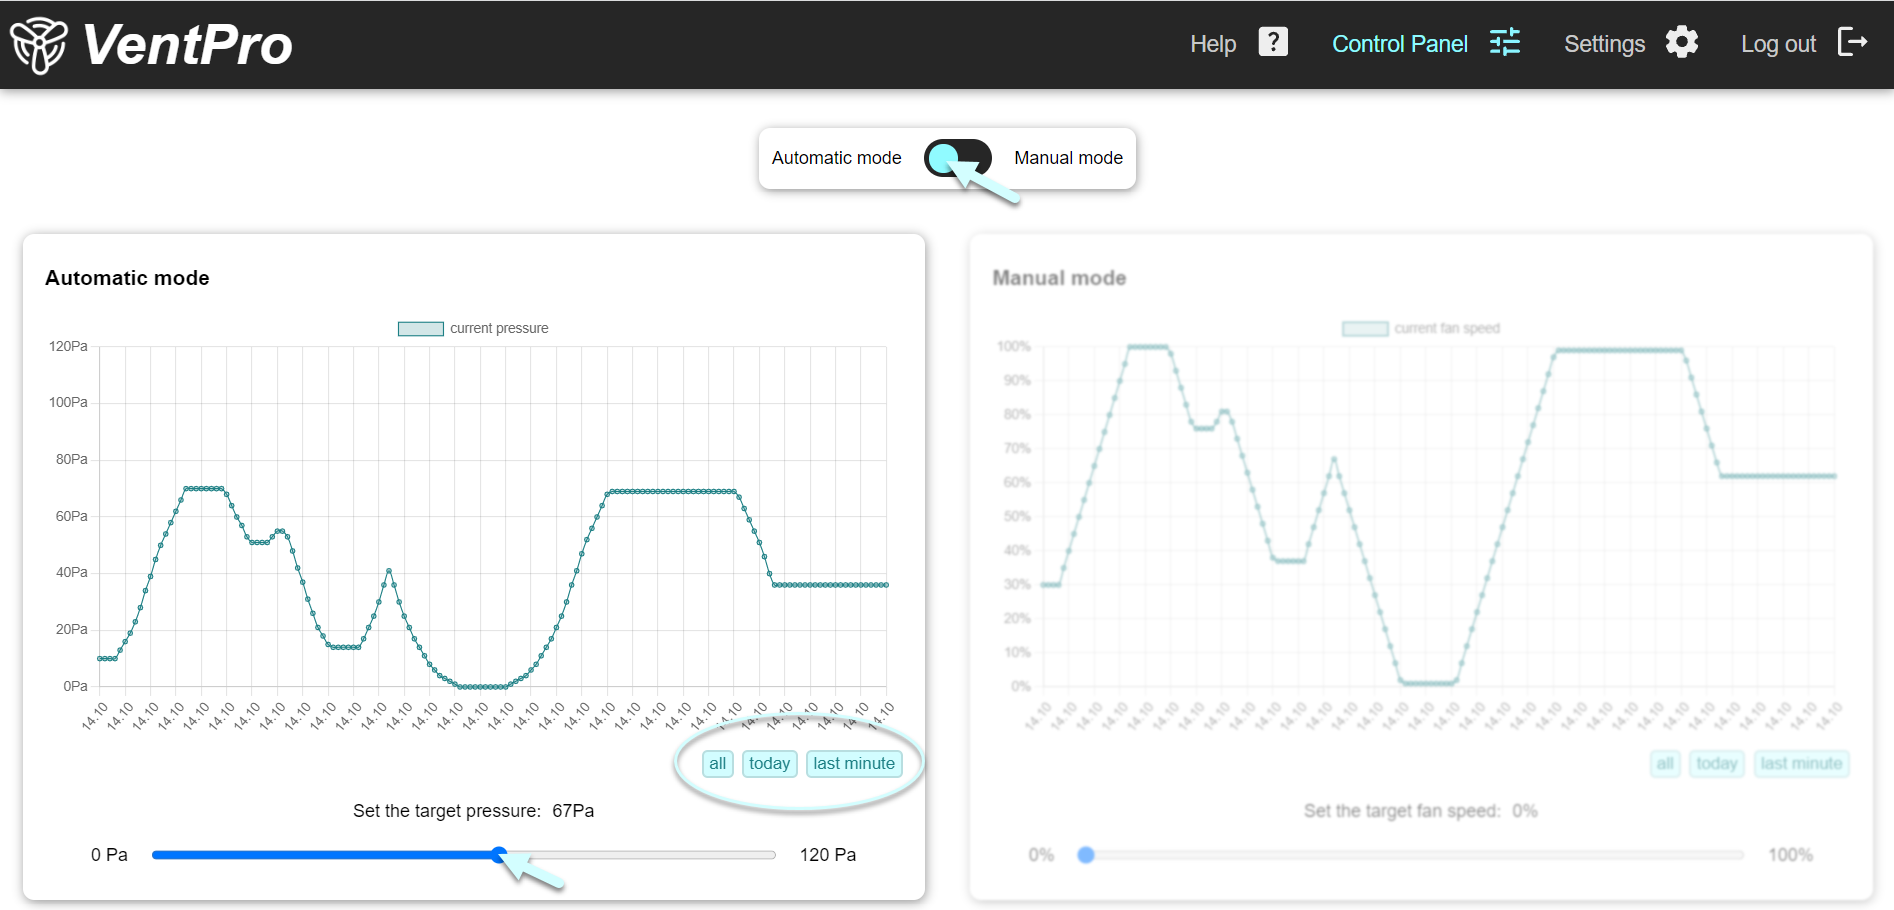
\includegraphics[width=1.0\textwidth]{img/Picture4}
\caption{Automatic mode}
\label{fig:picture_4}
\end{figure}
\vspace{0.3cm}

\begin{enumerate}[wide,  labelwidth=0.3cm,  labelindent=0pt, leftmargin=0.5cm]
\item In order to interact with the automatic mode of the website, click the turquoise and black toggle button in the middle of the website. The turquoise ball should be headed to the left side as displayed in figure \ref{fig:picture_4}.
\item If successful, the page should look like in figure \ref{fig:picture_4}.
\end{enumerate}

When the automatic mode is activated, you can set the pressure of the ventilator and see how this
impacts the current state of the graph.

\subsection*{Understanding the graph}

The x-axis of the automatic mode shows the time. When the manual mode is activated, you can set the pressure of the ventilator and see how this impacts the current state of the graph. By clicking the “today” button underneath the x-axis you can change the time interval to 24 hours. The “last minute” button changes the x-axis time interval to the last 60 seconds. The y-axis of the graph is the pressure measured in Pascal (Pa). The range of the graphs is 0Pa to 120Pa. To see the pressure at a specific point in time, hover over a data point in the graph. A black coloured box with information about the current pressure of the specific data
point is displayed (figure \ref{fig:picture_5}).

\subsection*{Set the target pressure}

With the scroll bar below the graph the target pressure can be set. To do so you have to click the grey ball on the scroll bar and move it. If you move it to the left the pressure decreases. Move the ball to the right to increase the pressure. The current target pressure is displayed next to “Set the target pressure:” above the scroll bar (figure \ref{fig:picture_4}).



\section{Manual mode}
\label{sec:manual_mode}

\begin{figure}[h]
\centering
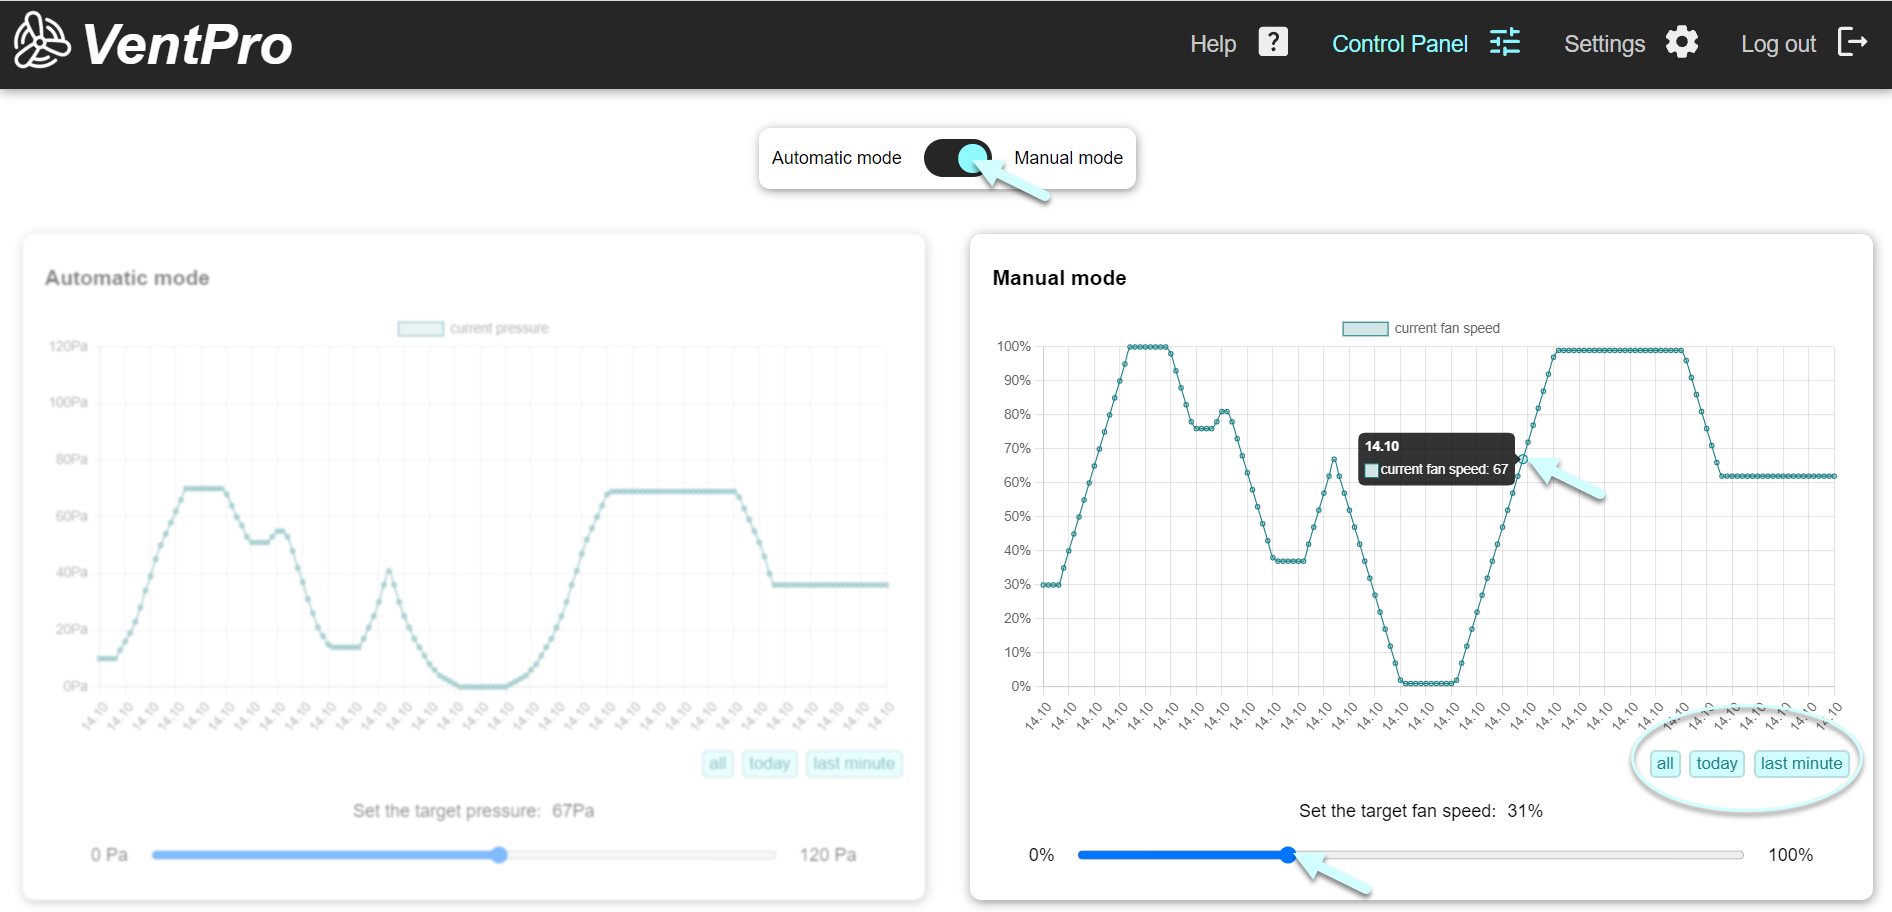
\includegraphics[width=1.0\textwidth]{img/Picture5}
\caption{Manual mode}
\label{fig:picture_5}
\end{figure}
\vspace{0.3cm}

\begin{enumerate}[wide,  labelwidth=0.3cm,  labelindent=0pt, leftmargin=0.5cm]
\item In order to interact with the manual mode of the website, click the turquoise and black toggle button in the middle of the website. The turquoise ball should be headed to the right side as displayed in figure \ref{fig:picture_5}.
\item If successful, the page should look like in fiure \ref{fig:picture_5}.
\end{enumerate}

When the manual mode is activated, you can adjust the speed of the ventilator and see how this
impacts the current state of the graph.

\subsection*{Understanding the graph}

The x-axis of the manual mode shows the time. In the default state the “all” button is preselected, showing data for the entire time the fan has been active, displayed in days. By clicking the “today” button underneath the x-axis you can change the time interval to 24 hours. The “last minute” button changes the x-axis time interval to the last 60 seconds. The y-axis of the graph is the fan speed displayed in percent. It ranges from 0\% to 100\% in the “all” graph and 0\% to 100\% in tthe graphs. To see the fan speed at a specific point in time, hover over a data point in the graph. A black coloured box with information about the current speed of the specific data point is displayed (figure \ref{fig:picture_5}).

\subsection*{Set the target fan speed}

With the scroll bar below the graph the target speed can be set. To do so you have to click the grey ball on the scroll bar and move it. If you move it to the left the speed decreases. Move the ball to the right to increase the fan speed. The current target speed is displayed next to “Set the target fan speed:” above the scroll bar (figure \ref{fig:picture_5}).



\chapter{Settings}
\label{sec:settings}

The following chapter describes the “Settings” page as well as its features and how to use them. The “Settings” page is divided into three sections “Log in activity”, “Change your password” and “Add a new user”.



\section{Login activity}
\label{sec:login_activity}

The box on the left keeps track of your login activities. It displays a list with date and time of your logins to the website as well as your username. The list is sorted in descending order, starting with your latest login and ending with your first. The latest nine logins are shown at once. By clicking the arrows underneath the dataset, you can switch to prior login data (figure \ref{fig:picture_6}). 

\color{red}
Note! The admin sees all login activites of the website’s users.
\color{black}

\vspace{0.5cm}
\begin{figure}[h]
\centering
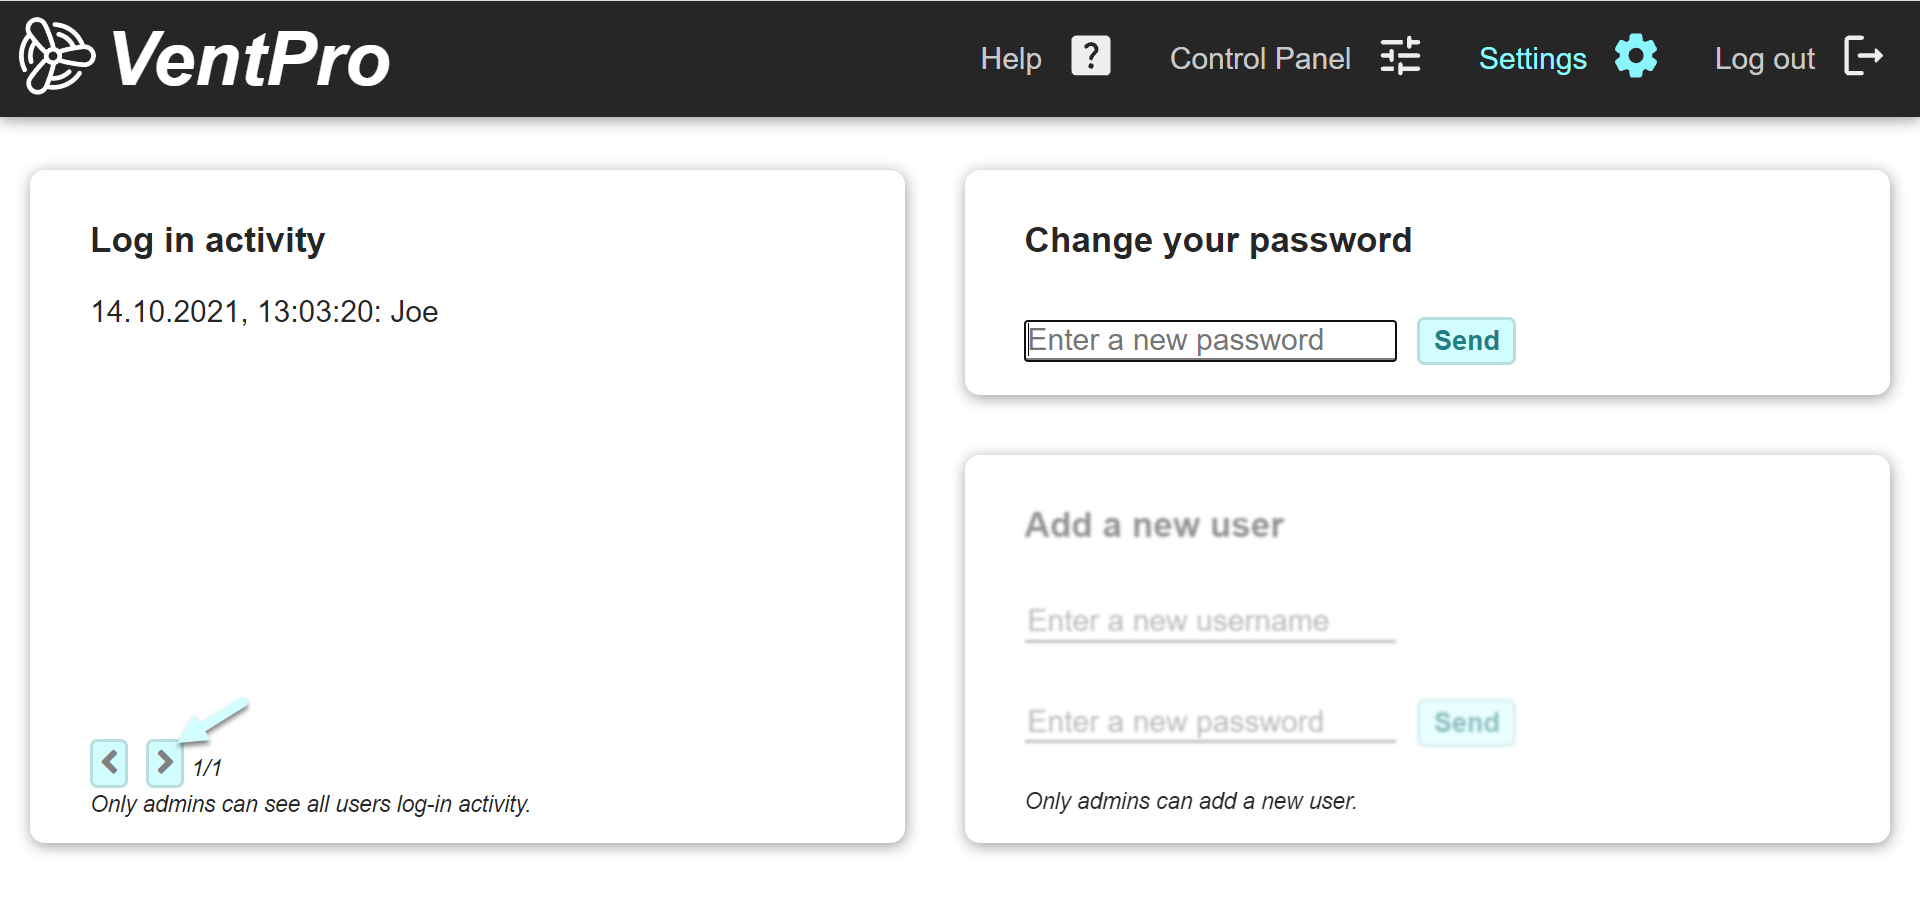
\includegraphics[width=1.0\textwidth]{img/Picture6}
\caption{Login activity}
\label{fig:picture_6}
\end{figure}


\newpage
\section{Change your password}
\label{sec:change_your_password}

The smaller box on the right-hand side is the place where you can change your password.

\begin{enumerate}[wide,  labelwidth=0.3cm,  labelindent=0pt, leftmargin=0.5cm]
\item Below the heading “Change your password” there is a field asking you to “Enter a new password”. Click into that field and type in a new password of your choice. Click the “Send” Button right next to the “Enter a new password” field to confirm your new password.\\
\color{red}
Note! Make sure to remember the new password for the next logins. The admin has no knowledge of your new password. The username given will remain the same.
\color{black}

\item If successful, the message “[OK] Your password has been changed successfully” will be displayed.
\item A login window pops up in the upper part of the screen and you are requested to login again with your new credentials.
\end{enumerate}



\section{Add a new user (Admin)}
\label{sec:add_a_new_user}

This section is relevant for admins only, because only admins are authorized to add a new user to the system. In the “Add a new user” box, in the right lower corner of the settings page, the admin can create new login accounts for the website.

\vspace{0.5cm}
\begin{figure}[h]
\centering
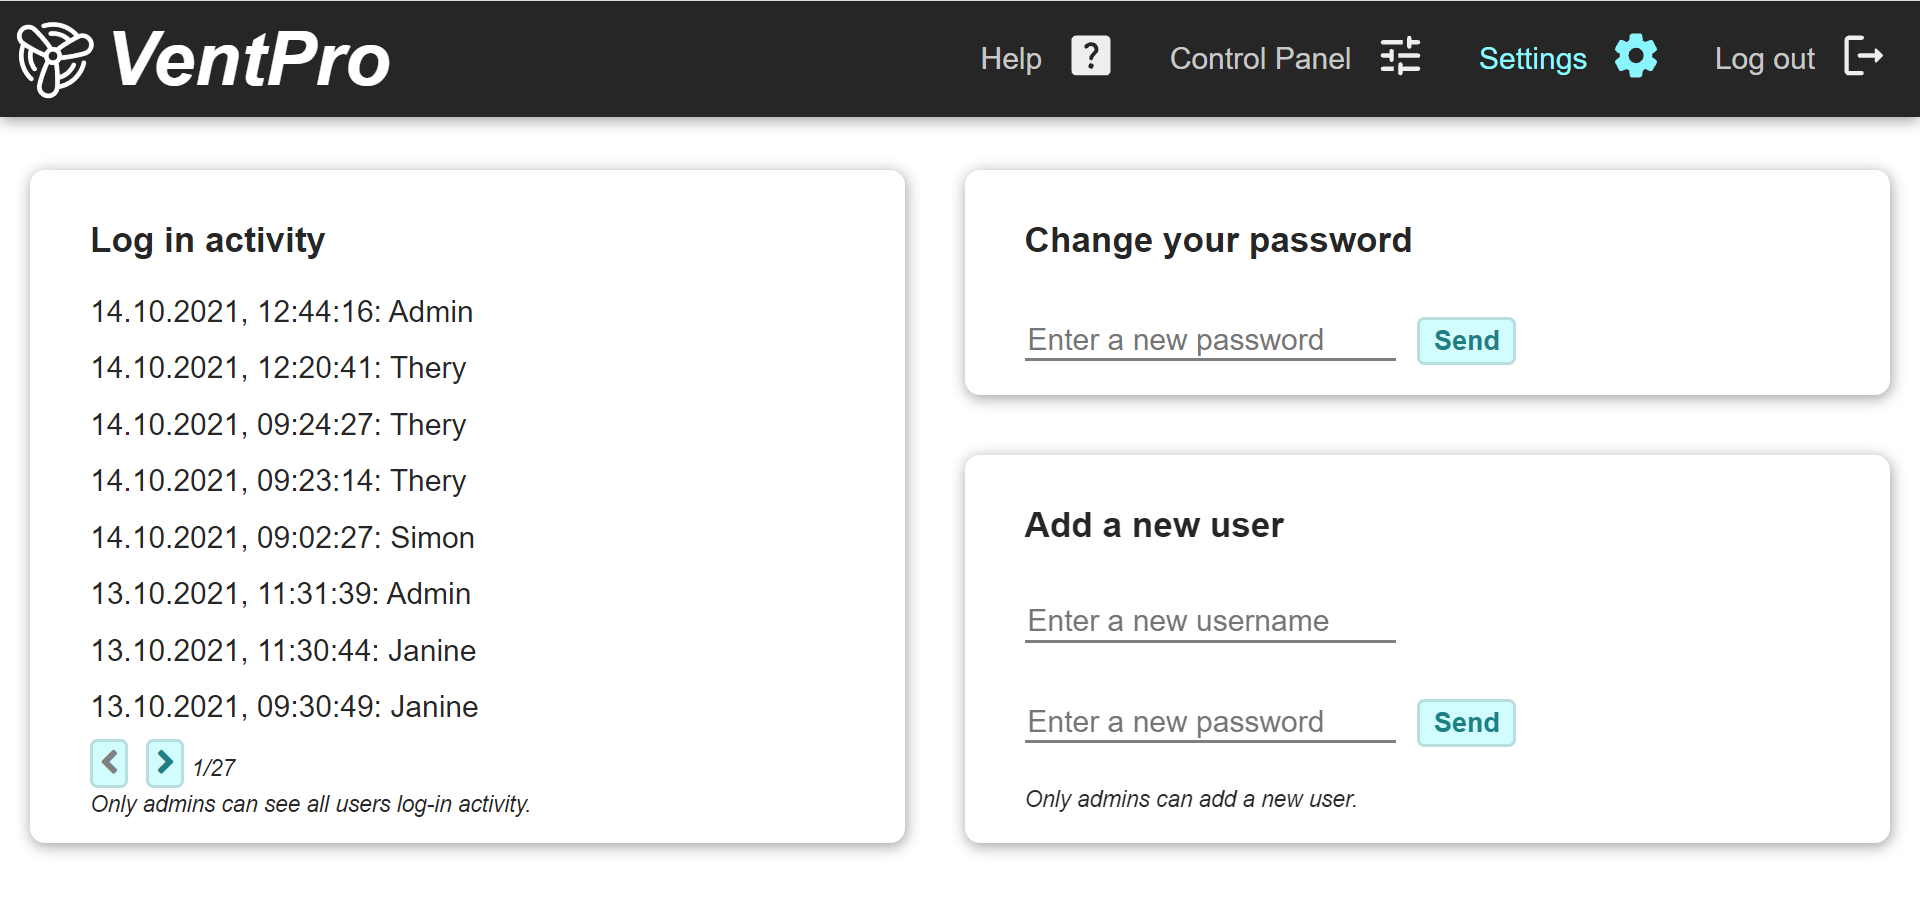
\includegraphics[width=1.0\textwidth]{img/Picture7}
\caption{Add a new user}
\label{fig:picture_7}
\end{figure}
\vspace{0.3cm}

\begin{enumerate}[wide,  labelwidth=0.3cm,  labelindent=0pt, leftmargin=0.5cm]
\item The admin has to select a username and a password for the new user.\\
\color{red}
Note! It is the admins responsibility to give the correct credentials to authorized users.
\color{black}
\item Type in the new username and password into the fields “Enter a new username” and “Enter a new password”.
\item Click the “Send” Button right next to the “Enter a new password” field to create a new user login account.
\item If successful, the message “[OK] The user was successfully added to the system” will be displayed.
\end{enumerate}



\chapter{Logout}
\label{sec:logout}

\begin{enumerate}[wide,  labelwidth=0.3cm,  labelindent=0pt, leftmargin=0.5cm]
\item By clicking “Log out” (figure \ref{fig:picture_8}) in the menu at the top of the screen, you can logout from the website.
\item If the logout was successful, the logout page is displayed as in figure \ref{fig:picture_9}.
\item If you want to login again, it is possible by clicking on “Log in” in the top right corner of the website
or by clicking “Log back in” in the middle of the website. You can also follow the steps described in the section “Log in”.
\end{enumerate}

\vspace{0.5cm}
\begin{figure}[h]
\centering
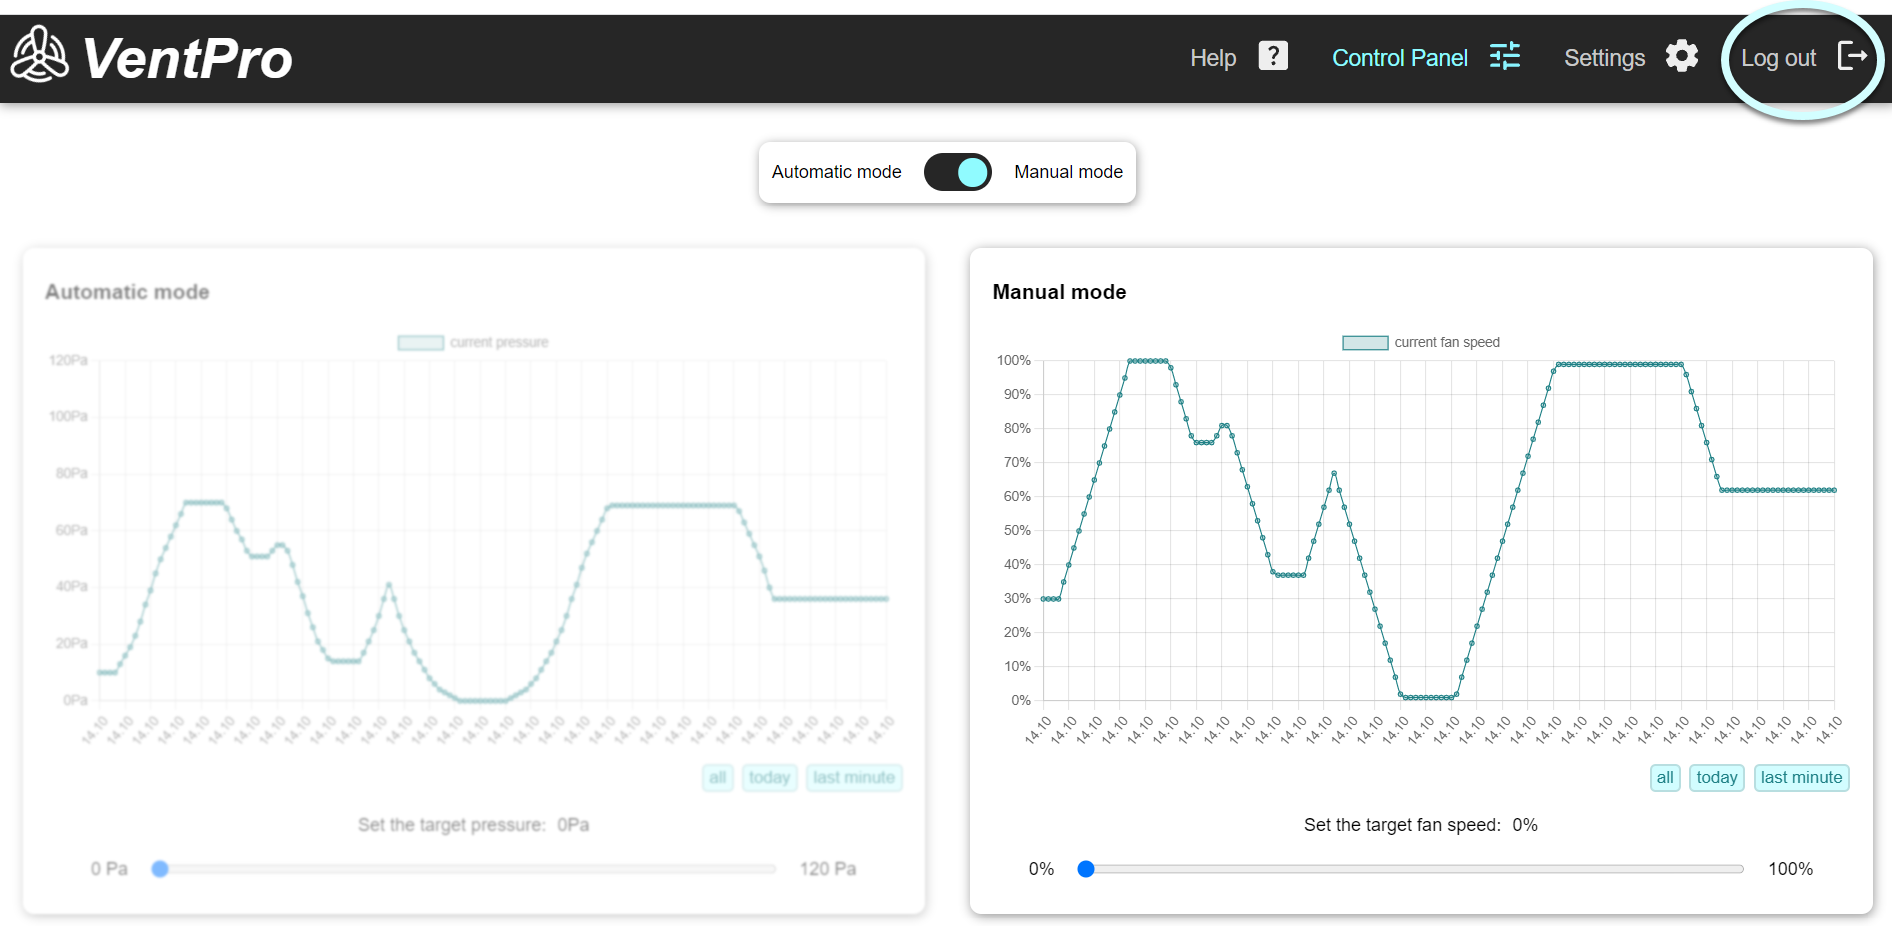
\includegraphics[width=1.0\textwidth]{img/Picture8}
\caption{Logout}
\label{fig:picture_8}
\end{figure}

\begin{figure}[h]
\centering
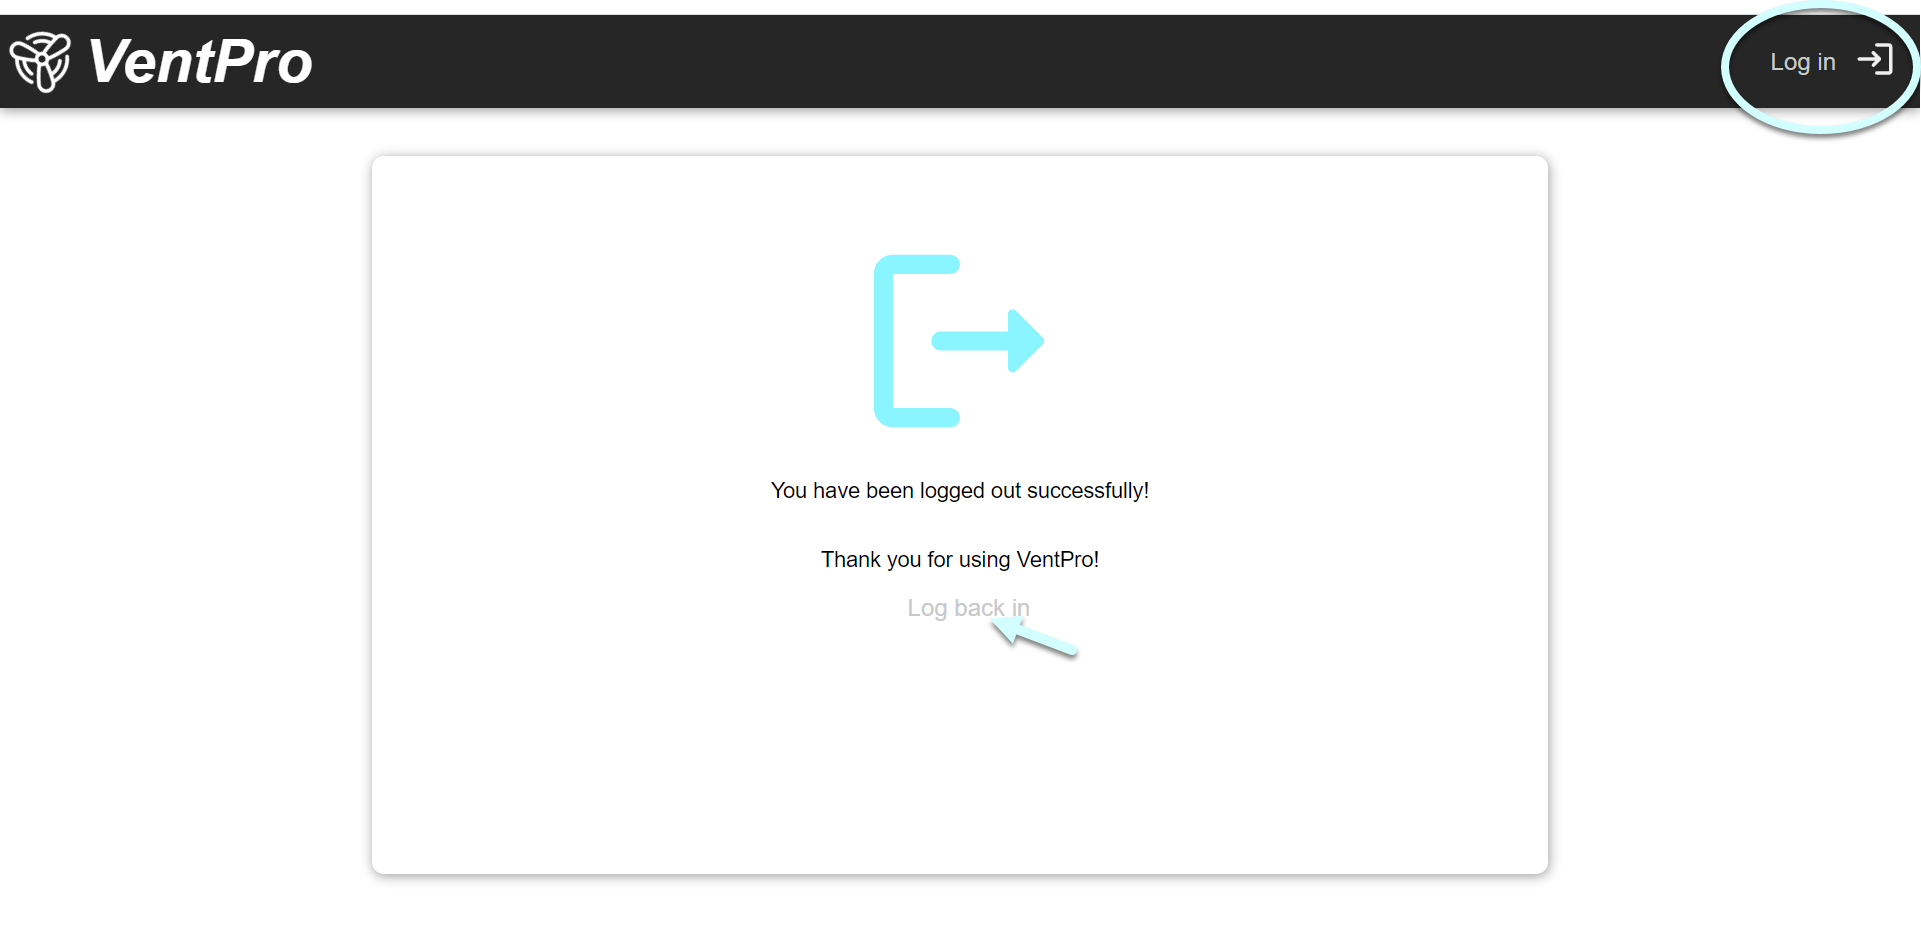
\includegraphics[width=1.0\textwidth]{img/Picture9}
\caption{Log back in}
\label{fig:picture_9}
\end{figure}
